\documentclass[final]{beamer}

\mode<presentation>
{
  \definecolor{berkeleyblue}{HTML}{003A70}
  \definecolor{berkeleygold}{HTML}{F2A900}
%http://www.berkeley.edu/brand/img/downloads/UCB%20Brand%20Guidelines_FINAL_small.pdf
  \usetheme{I6dv}      % or try Darmstadt, Madrid, Warsaw, ...
  %\usecolortheme{dove} % or try albatross, beaver, crane, ...
  \setbeamercolor{structure}{fg=berkeleygold,bg=berkeleyblue}
  \setbeamercolor{palette primary}{fg=berkeleyblue,bg=berkeleygold} % changed this
  \setbeamercolor{palette secondary}{bg=berkeleyblue,fg=white} % changed this
  \setbeamercolor{palette tertiary}{bg=berkeleyblue,fg=white} % changed this
\setbeamercolor{bibliography item}{bg=white,fg=black}
\setbeamercolor{bibliography entry author}{bg=white,fg=black}
\setbeamercolor{bibliography entry journal}{bg=white,fg=black}
\setbeamercolor{bibliography entry note}{bg=white,fg=black}
  \usefonttheme{structurebold}  % or try serif, structurebold, ...
  \useinnertheme{circles}
  \setbeamertemplate{navigation symbols}{}
  \setbeamertemplate{footline}[title]{}
  \setbeamertemplate{footline}[author]{}
  \usebackgroundtemplate{
%  \tikz[overlay,remember picture] %Can insert a Berkeley watermark
%  \node[opacity=1, at=(current page.south west),anchor=south west, inner sep=2pt] {
%    \includegraphics[height=.5in,width=.5in]{img/ucseal_540_139.eps}};
}
}
\usepackage[sorting=none]{biblatex} 
  \usepackage{ragged2e}
  \usepackage{type1cm}
  \usepackage{calc} 
  \usepackage{times}
  \usepackage{amsmath,amsthm, amssymb, latexsym}
%  \boldmath
  \usepackage[english]{babel}
  \usepackage[latin1]{inputenc}
  \usepackage[orientation=landscape,size=a0,scale=1.4,debug]{beamerposter}
  \graphicspath{{img/}}
  %\title[Fancy Posters]{Making Really Fancy Posters with \LaTeX}
  %\author[Dreuw \& Deselaers]{Philippe Dreuw and Thomas Deselaers}
  %\institute[University of California, Berkeley]{Department of Nuclear Engineering}
  \newcommand{\footlinetext}{}

% Transport equation stuff
\newcommand{\Sn}{\ensuremath{S_N}}
\newcommand{\Macro}{\ensuremath{\Sigma}}

\newcommand{\vOmega}{\ensuremath{\hat{\Omega}}}
\newcommand{\Ye}[2]{\ensuremath{Y^e_{#1}(\vOmega_#2)}}
\newcommand{\Yo}[2]{\ensuremath{Y^o_{#1}(\vOmega_#2)}}

\newcommand{\ve}[1]{\ensuremath{\mathbf{#1}}}

\setbeamertemplate{bibliography item}[text]
\addbibresource{2015-bascd.bib}
%\bibliographystyle{amsalpha}

\title[RQI with MGE]{RQI with a Multigrid in Energy Preconditioner for Massively Parallel Neutron Transport}
\author[R.N.\ Slaybaugh et al.]{R.N.\ Slaybaugh$^{1}$, T.M.\ Evans$^{2}$, G.G. Davidson$^{2}$, S.P.\ Hamilton$^{2}$}
  \institute[UC Berkeley]{$^{1}$Department of Nuclear Engineering, University of California, Berkeley\\
  $^{2}$Radiation Transport Group, Oak Ridge National Laboratory}
  \date{December 11, 2015}

\begin{document}
	\begin{frame}{}
%    \maketitle

%%%%%%%%%%%%%%
% FIRST COLUMN
%%%%%%%%%%%%%%

  		\begin{columns}[t]
    		\begin{column}{.3\linewidth}
    			\vfill
    			\begin{block}{\large Motivation}
      			\begin{itemize}
			\item{Nuclear reactor design, shielding, nuclear security}
			\item{3D deterministic calculations need fine resolution in space, 
			      energy, and angle}
			\item{Need to use supercomputing architectures effectively}
			\item{Three complimentary methods: multigroup (MG) block Krylov, 
			      Rayleigh quotient iteration (RQI), multigrid in energy (MGE)
			      preconditioner}
			\end{itemize}
    			\end{block}
    	\vfill
    			\begin{block}{\large Boltzmann Transport Equation}
			\begin{itemize}
	 		\item{Solve for $\psi$, the angular neutron flux (n/cm$^2$-s-steradian)}
	 		\begin{equation}
	 		  \ve{L}\psi = \ve{MS}\phi + \frac{1}{k}\ve{M}\chi \ve{f}^{T}\phi	                
	 		  \label{eq:eigenvalue}
	 		\end{equation}	 		
	 		\item{Collocation method in angle: $\phi = \mathbf{D} \psi$ (n/cm$^2$-s)}
	 		\item{$\ve{L}$ is the $\vOmega \cdot \nabla + \Macro_t$ operator; $\ve{M}$
	 		 projects $\phi$ onto discrete angles; $\ve{S}$
	 		 is the scattering matrix; $\ve{f}$ contains the fission source, 
	 		 $\nu \Macro_{f}$; and $k$ is the asymptotic ratio of the number of 
	 		 neutrons in one generation to the next}
	 		\item{Rearrange \eqref{eq:eigenvalue}; define $\ve{T} = \ve{DL}^{-1}$ 
	 		 and $\ve{F} = \chi \ve{f}^{T}$ \cite{denovo}}:
            \begin{equation}
              (\ve{I} - \ve{TMS})\phi = \frac{1}{k} \ve{TMF} \phi
              \label{eq:OperatorEvalForm}
            \end{equation}
            \item{Get series of ``within-group'' eqns., each only a function of space
             and angle}
            \item{Groups can be coupled by scattering from low to higher energy
             $\rightarrow$ iterative ``multigroup'' solves over the coupled portion needed}
			\end{itemize}
    			\end{block}
    	\vfill
        	\begin{block}{\large Multigroup Block Krylov}		
		\begin{itemize}
		\item{Groups historically solved in series with Gauss Seidel} 
			\begin{figure}[h!]
			\centering
	      		\includegraphics{block-krylov.png}
			%\caption{MG Krylov group blocking}
			\end{figure}
		\item{Solve downscatter groups individually}
		\item{Solve upscatter block together with multi-group-sized iteration vector 
		      in GMRES}
		\item{Enables parallelization in energy (``multisets") \cite{Davidson2013}}
		\end{itemize}
        	\end{block}
    	\end{column}

%%%%%%%%%%%%%%%
% SECOND COLUMN
%%%%%%%%%%%%%%%

      	\begin{column}{.3\linewidth}
            \begin{block}{Rayleigh Quotient Iteration}
	\begin{itemize}
	\item{``Virtual collisions" are scattering reactions that preserve neutron energy and direction}
		\begin{itemize}
		\item{No impact on final outcome, any number can ``happen"}
		\end{itemize}
	\item{Materials' total cross sections can be adjusted by adding arbitrary virtual collision cross section:}
		\begin{equation*}
		\Sigma'_{\mathrm{tot,m}}(E) = \Sigma_{\mathrm{tot,m}}(E) + \Sigma_{\mathrm{0,m}}(E)
		\end{equation*}
	\item{With this, global majorant cross section can be assigned:}
		\begin{equation*}
		\begin{aligned}
		\Sigma_{\mathrm{maj}}(E) &=\Sigma'_{\mathrm{tot,1}}(E) = \Sigma'_{\mathrm{tot,2}}(E) = \ldots = \Sigma'_{\mathrm{tot,M}}(E) \\
		& = \mathrm{max}\{\Sigma_{\mathrm{tot,1}}(E), \Sigma_{\mathrm{tot,2}}(E),\ldots, \Sigma_{\mathrm{tot,M}}(E)\}
		\end{aligned}
		\end{equation*}
		\item{Path lengths sampled with majorant cross section valid globally}
		\item{Rejection sampling carried out for each collision}
		\item{Collision point accepted with probability}
		\begin{equation*} 
		P_{\mathrm{col}}(E) = \Sigma_{\mathrm{tot,col}}(E)/\Sigma_{\mathrm{maj}}(E)
		\end{equation*}
		\item{If point rejected, collision considered virtual and random walk 
		continues by sampling new path length \cite{serpent}}
	\end{itemize}
            \end{block}
		\vfill
        	\begin{block}{\large Run Parameters}
          		\begin{itemize}
			\item{MCNP and Serpent runs done on server with two AMD Opteron 6128 
			Magny-Cours processors}
			\item{WARP runs done with NVIDIA GeForce GTX TITAN Black GPU}
			\item{20 inactive cycles, 40 active cycles, 100 000 histories}
			\item{Vacuum boundary conditions, ENDF/B-VII data at 300K}
			\end{itemize}
        	\end{block}
			\vfill
		\begin{block}{\large Results - Jezebel}
\begin{columns}
	\column{0.3\linewidth}
	\begin{figure}[h!]
	
\includegraphics[width=4in]{img/jezebel.png}
	\caption{\footnotesize Plot of ``jezebel" geometry configuration, a bare Pu-239 sphere
	with radius 5.1 cm.}
	\end{figure}
	\column{0.7\linewidth}
	\begin{table}[h]
	\begin{tabular}{ll}
	\multicolumn{2}{c}{Single-run Multiplication Factors} \\ \hline
	MCNP5, 1.60 & $k_{\mathrm{eff}} = 1.027509 \pm 0.0005$ \\
	Serpent 1.1.19 & $k_{\mathrm{eff}} = 1.02787\hspace*{0.5em}\pm 0.00082$ \\
	WARP (RT) & $k_{\mathrm{eff}} = 1.028425 \pm 0.00068609$ \\
	WARP (DT) & $k_{\mathrm{eff}} = 1.027071 \pm 0.00058248$
	\end{tabular}
	\end{table}
	\begin{table}[h]
	\begin{tabular}{ll}
	\multicolumn{2}{c}{Runtimes} \\ \hline
	MCNP5, 1.60 & 0.94 min \\
	Serpent 1.1.19 & 0.934333 min \\
	WARP (RT) & 0.141333 min \\ %8.48 s
	WARP (DT) & 0.194833 min %11.69 s
	\end{tabular}
	\end{table}
\end{columns}
	\begin{itemize}
	\item Delta-tracking slower than ray tracing in WARP
		\begin{itemize}
		\item Additional OptiX trace necessary
		\end{itemize}
	\item Accuracy retained with delta-tracking
	\end{itemize}
		\end{block}
	\vfill
      \end{column}

%%%%%%%%%%%%%%
% THIRD COLUMN
%%%%%%%%%%%%%%

      \begin{column}{.3\linewidth}
		\begin{block}{Results - Jezebel with Artificial Boundary}
\begin{columns}
	\column{0.3\linewidth}
	\begin{figure}[h!]
	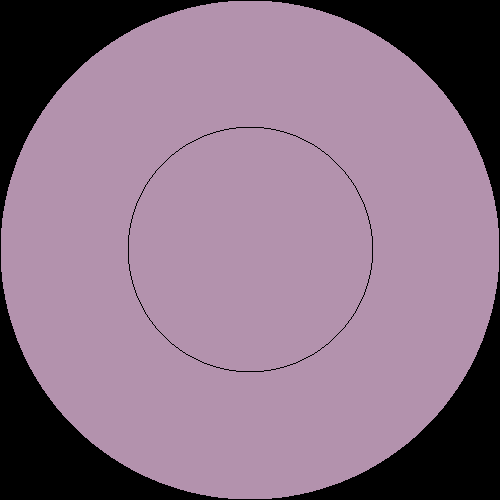
\includegraphics[width=4in]{img/jezebel-shells.png}
	\caption{Plot of ``jezebel" configuration with an inserted artificial boundary.}
	\end{figure}
	\column{0.7\linewidth}
	\begin{itemize}
	\item{Artificial boundary put in place to test different method speeds}
	\item{Verify that delta-tracking performs correctly with boundary}
	\end{itemize}
	\begin{table}[h]
	\begin{tabular}{ll}
	\multicolumn{2}{c}{Single-run Multiplication Factors} \\ \hline
	MCNP5, 1.60 & $k_{\mathrm{eff}} = 1.027472 \pm 0.0004$ \\
	Serpent 1.1.19 & $k_{\mathrm{eff}} = 1.02815\hspace*{0.5em}\pm 0.00089$ \\
	WARP (RT) & $k_{\mathrm{eff}} = 1.027211 \pm 0.00061316$ \\
	WARP (DT) & $k_{\mathrm{eff}} = 1.027071 \pm 0.00058248$
	\end{tabular}
	\end{table}
	\begin{table}[h]
	\begin{tabular}{ll}
	\multicolumn{2}{c}{Runtimes} \\ \hline
	MCNP5, 1.60 & 0.91 min \\
	Serpent 1.1.19 & 0.953333 min \\
	WARP (RT) & 0.162833 min \\ %9.77 s
	WARP (DT) & 0.198 min %11.88 s
	\end{tabular}
	\end{table}
\end{columns}
		\end{block}
			\vfill
        	\begin{block}{\large Future Work}
          		\begin{itemize}
          			\item Test configurations with material heterogeneities
				\item{Retest delta-tracking if WARP moves to universe-based geometry similar to MCNP and Serpent}
          			\item Investigate use of path-dependent majorant calculation
          		\end{itemize}
        	\end{block}
			\vfill
        	\begin{block}{\large References}
			\printbibliography
        	\end{block}
			\vfill
        	\begin{block}{\large Acknowledgements}
		\justifying
This research used resources of the Oak Ridge Leadership Computing Facility at the Oak Ridge National Laboratory, which is supported by the Office of Science of the U.S.\ Department of Energy under Contract No. DE-AC05-00OR22725. Additional thanks to the Rickover Fellowship Program in Nuclear Engineering sponsored by Naval Reactors Division of the U.S.\ Department of Energy. This fellowship sponsored the work from which this work is derived. 
        	\end{block}
      \end{column}
    \end{columns}
  \end{frame}
\end{document}

%    			\begin{block}{\large Fontsizes}
%      				\centering
%      				{\tiny tiny}\par
%      				{\scriptsize scriptsize}\par
%      				{\footnotesize footnotesize}\par
%      				{\normalsize normalsize}\par
%      				{\large large}\par
%      				{\Large Large}\par
%      				{\LARGE LARGE}\par
%      				{\veryHuge VeryHuge}\par
%      				{\VeryHuge VeryHuge}\par
%      				{\VERYHuge VERYHuge}\par
%    			\end{block}

%%%%%%%%%%%%%%%%%%%%%%%%%%%%%%%%%%%%%%%%%%%%%%%%%%%%%%%%%%%%%%%%%%%%%%%%%%%%%%%%%%%%%%%%%%%%%%%%%%%%
%%% Local Variables: 
%%% mode: latex
%%% TeX-PDF-mode: t
